\documentclass[10pt,utf8]{beamer}

\mode<presentation> {
%  \usetheme{Boadilla}
  \usetheme{Madrid}
%	\usetheme{Fzu}
  \setbeamercovered{transparent}
}

\usepackage{palatino}
\usepackage{graphicx}
\usepackage{array}
\usepackage{color}
\usepackage{subfigure}
\usepackage{colortbl}
\usepackage{amsmath}
\usepackage{hyperref}
\usepackage{listings}
\usepackage{fancyvrb}

\setbeamertemplate{caption}{\raggedright\insertcaption\par} %turn off caption prefix ("Figure")

\title{OpenJDK project Loom}
\author{Vojtech Juranek}
\institute[Red Hat]{oVirt storage team}
\date{??.~11.~2020}

\lstdefinestyle{java}{
	basicstyle          = \large\ttfamily,
	language            = java,
	numbers             = left,
	numberstyle         = \small,
	stepnumber          = 1,
	numbersep           = 5pt,
	backgroundcolor     = \color{white},
	showspaces          = false,
	showstringspaces    = false,
	showtabs            = false,
	frame               = single,
	tabsize             = 2,
	captionpos          = b,
	breaklines          = true,
	breakatwhitespace   = false,
	morestring          = [b]",
	stringstyle         = \color{blue},
	keywordstyle        = \color{magenta},
	commentstyle        = \color{gray},
	identifierstyle     = \color{black},
	moredelim           = **[is][\bfseries]{`}{`},
	moredelim           = **[is][\color{magenta}]{$}{$}, 
	fancyvrb            = true,
}


\begin{document}

\begin{frame}
	\titlepage
\end{frame}

\begin{frame}[fragile]
    \frametitle{Java concurrency}
    Low-level thread: \texttt{java.lang.Threads} class and \texttt{java.lang.Runnable}.
    \begin{lstlisting}[style=java]
Runnable task = new MyRunnable();
Thread thread = new Thread(task);
thread.start();
    \end{lstlisting}
\end{frame}

\begin{frame}[fragile]
    \frametitle{Java concurrency}
    High-level Executor framework:
    \begin{lstlisting}[style=java]
Runnable task = new MyRunnable();
ExecutorService executor = Executors.newFixedThreadPool(NUM_THREADS);
executor.execute(task);
    \end{lstlisting}
    
    \vspace{0.5cm}
    \begin{lstlisting}[style=java]
Runnable task = new MyRunnable();
ExecutorService executor = Executors.newFixedThreadPool(NUM_THREADS);
Future<?> f = executor.submit(task);
    \end{lstlisting}
\end{frame}

\begin{frame}[fragile]
    \frametitle{Java concurrency}
    Async. constructs added in Java 8 (e.g. CompletableFuture):
    \begin{lstlisting}[style=java]
public String myFunction(int a) {...}
CompletableFuture<String> cf = CompletableFuture.supplyAsync(() -> myFunction(10));
cf.thenAccept(result -> System.out.println(result));
    \end{lstlisting}
And many other ways how to run function asynchronously, e.g.:
    \begin{lstlisting}[style=java]
public String myFunction(int a) {...}
Stream.of(1, 2).parallel().forEach(i -> myFunction(i));
    \end{lstlisting}
\end{frame}

\begin{frame}[fragile]
    \frametitle{Asynchronous frameworks}
    \begin{itemize}
        \item \href{https://vertx.io/}{\textcolor{blue}{vert.x}}
        \item \href{https://netty.io/}{\textcolor{blue}{Netty}\textcolor{black}}
        \item ...
    \end{itemize}

    \vspace{0.5cm}

Vert.x example:
    \begin{lstlisting}[style=java]
vertx.createHttpServer().requestHandler(r -> {
  r.response()
    .putHeader("content-type", "text/plain")
    .end("Hello from Vert.x!");
}).listen(8080);
    \end{lstlisting}
\end{frame}


\begin{frame}
  \frametitle{Synchronous vs. asynchronous}
  \begin{columns}
        \column{0.6\textwidth}
            Synchronous:
            \begin{itemize}
                \item Simple to reason about it.
                \item Blocking.
                \item Less scalable.
            \end{itemize}
            
            \vspace{0.5cm}
            
            Asynchronous:
            \begin{itemize}
                \item Harder to reason about it.
                \item Better scales.
                \item To get maximum benefit from it, all parts have to be asynchronous.
                \item Can be problematic to make it working with legacy synchronous code.
            \end{itemize}
            
        \column{0.4\textwidth}
            \begin{figure}
                \centering
                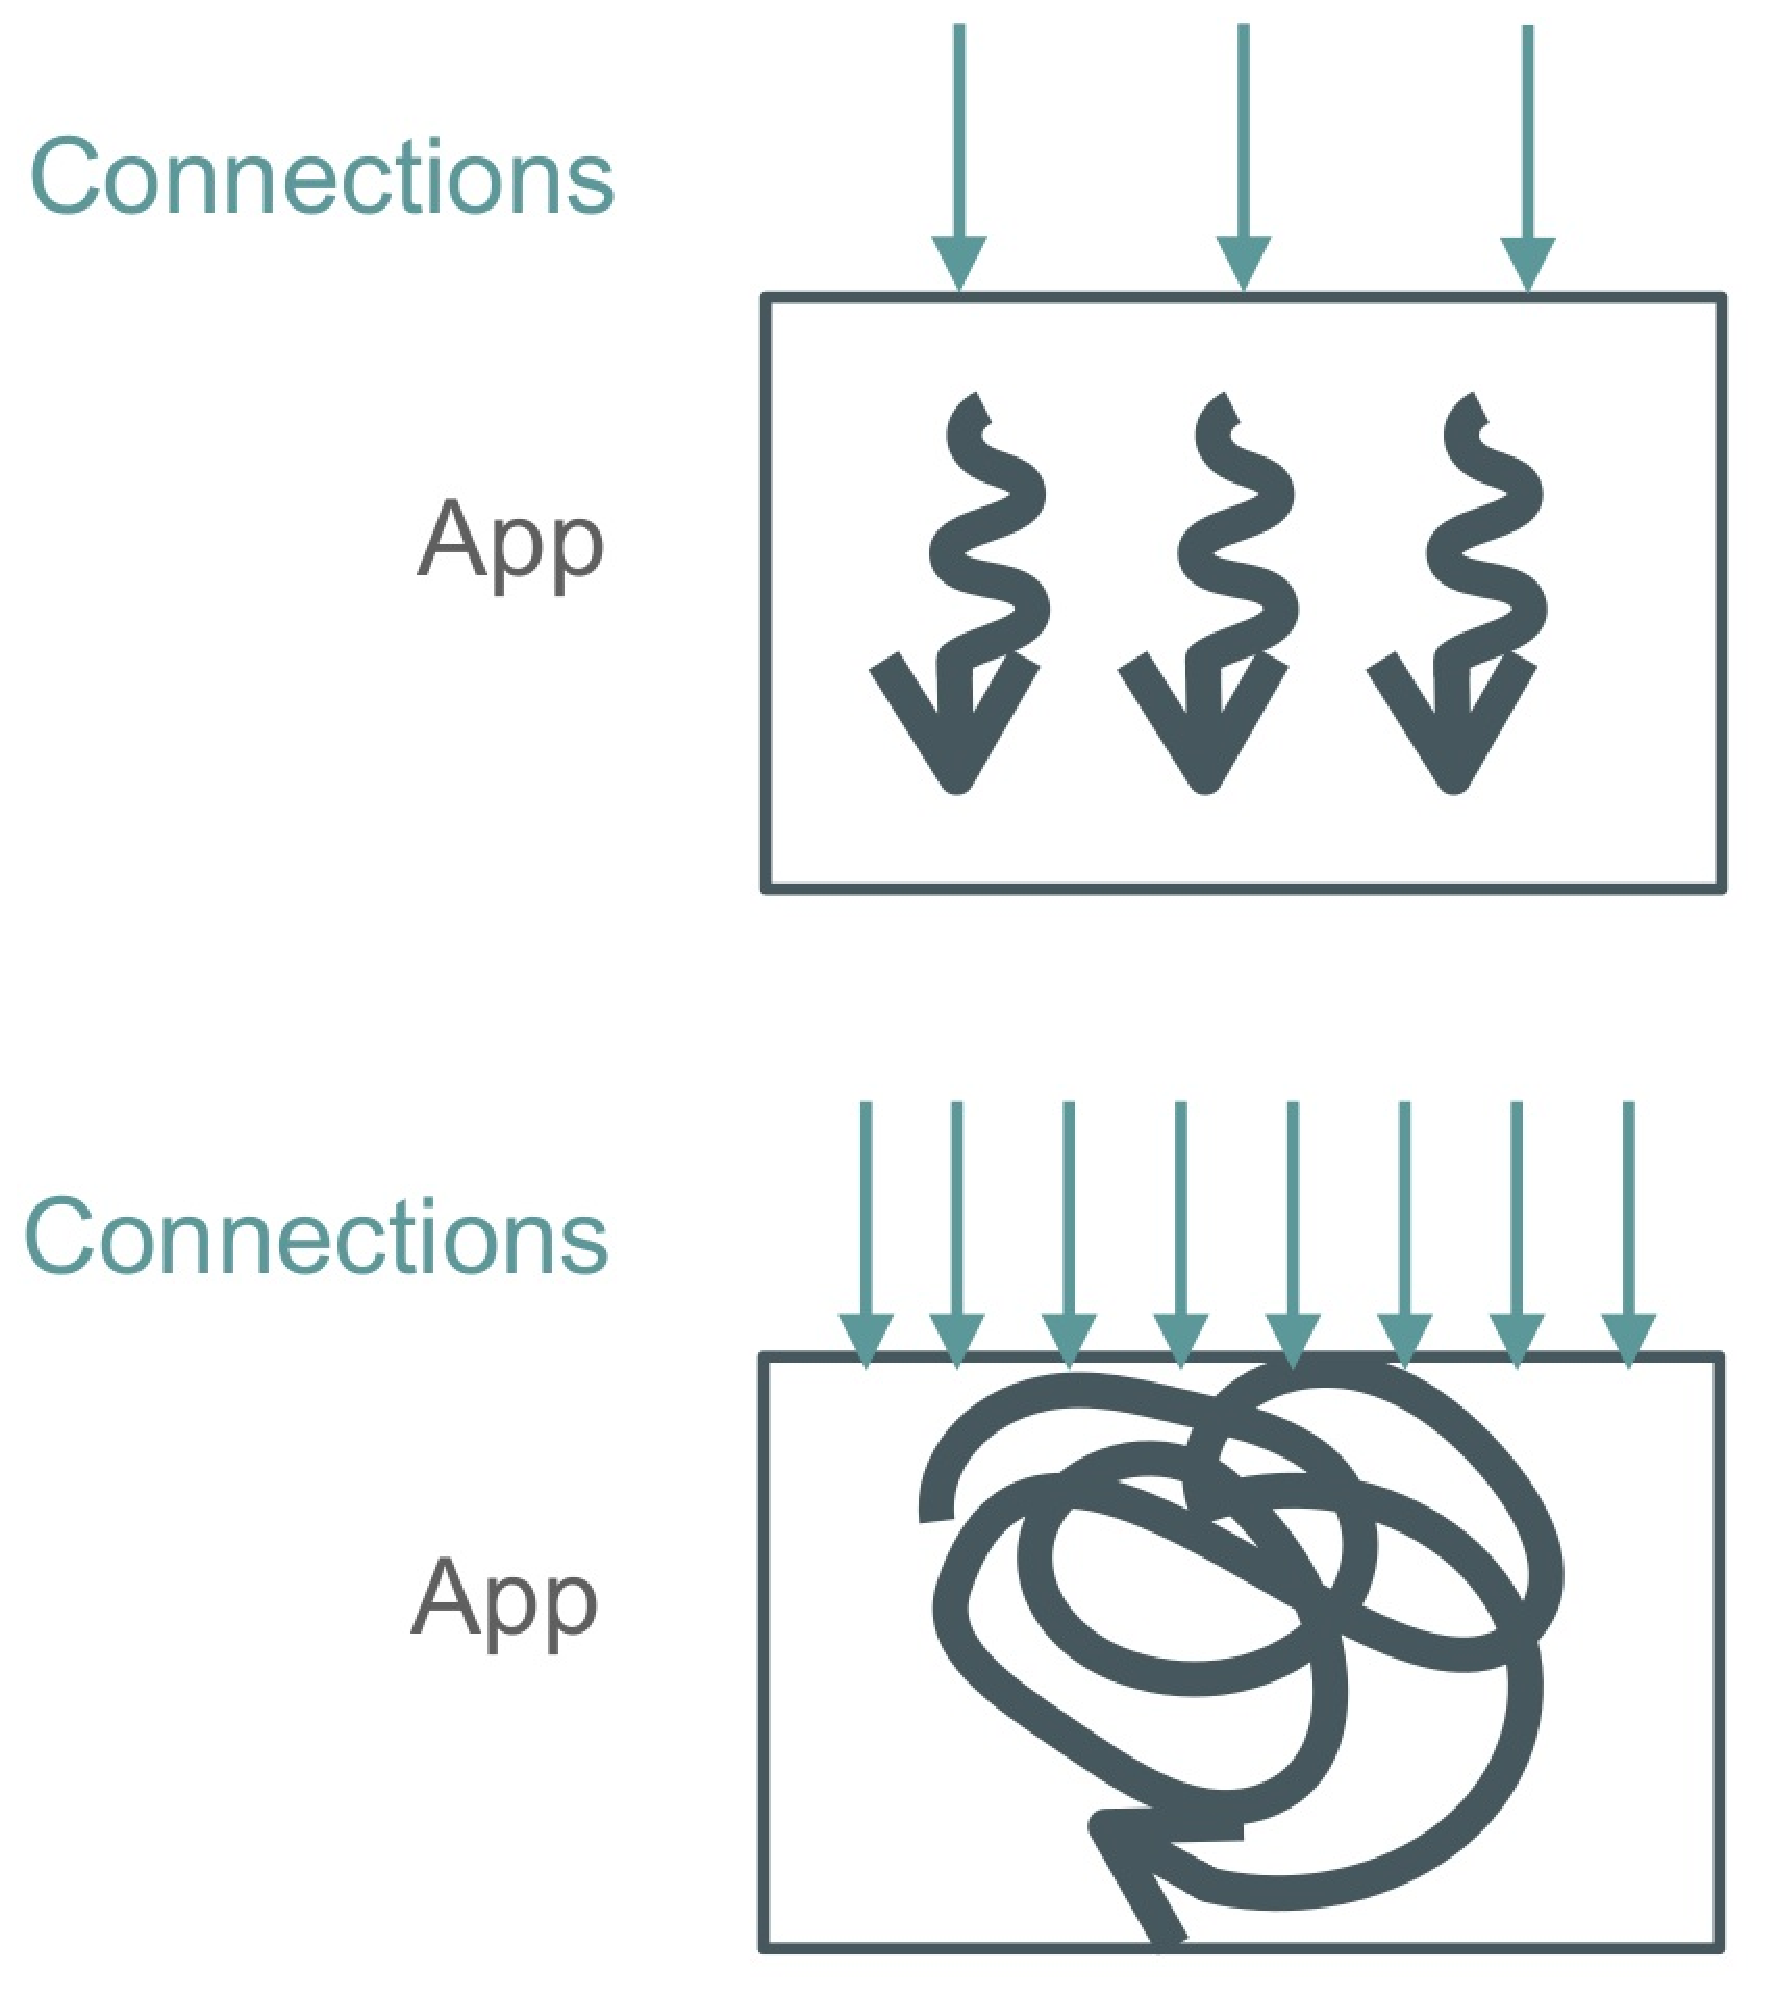
\includegraphics[height=5cm]{./img/sync_vs_async.eps}
                \caption{\tiny{Source: \url{http://cr.openjdk.java.net/~alanb/loom/Devoxx2018.pdf}}}
            \end{figure}
    \end{columns}
\end{frame}

\begin{frame}[fragile]
    \frametitle{Handling error in async. code}
Netty example:
    \begin{lstlisting}[style=java]
ChannelFuture f = ctx.writeAndFlush(b);
f.addListener(writeFailed);

$private$ $final$ ChannelFutureListener writeFailed = (ChannelFuture future) -> {
    if (!future.isSuccess()) {
        future.cause().printStackTrace();
        future.channel().close();
    }
};
    \end{lstlisting}
\end{frame}

\begin{frame}
  \frametitle{Project Loom}
	\begin{itemize}
		\item \url{https://wiki.openjdk.java.net/display/loom/Main}
		\item Virtual threads
		\item Delimited continuations
		\item Tail-call elimination
	\end{itemize}
\end{frame}

\begin{frame}
  \frametitle{Virtual threads}
	\begin{itemize}
		\item Virtual threads cannot be suspended, resumed or stopped with the Thread suspend, resume and stop APIs.
		\item All virtual threads are in the same ThreadGroup.
	\end{itemize}
\end{frame}

\begin{frame}[fragile]
	\frametitle{Virtual threads}
	\begin{lstlisting}[style=java]
var thread = Thread.startVirtualThread(() -> System.out.println("Virtual thread!"));
thread.join();
	\end{lstlisting}
\end{frame}


\begin{frame}
  \frametitle{Virtual threads}
	\centering
	\huge{\textbf{Demo}}
\end{frame}

\begin{frame}
    \begin{itemize}
        \item \href{https://wiki.openjdk.java.net/display/loom/Main}{\textcolor{blue}{Project Loom web page}\textcolor{black}}
    \end{itemize}
\end{frame}


\end{document}
